%!TEX program=xelatex

\documentclass[11pt]{ctexart}  
\usepackage[top=2cm, bottom=2cm, left=2cm, right=2cm]{geometry}  
\usepackage{algorithm}  
\usepackage{algorithmicx}  
\usepackage{algpseudocode}  
\usepackage{amsmath}  
\usepackage{graphicx}
\usepackage{amsmath}
\usepackage{amssymb}


\floatname{algorithm}{算法}
\renewcommand{\algorithmicrequire}{\textbf{输入:}}  
\renewcommand{\algorithmicensure}{\textbf{输出:}} 

\title{密码学实验报告2}
\author{张天辰	17377321}

\makeatletter
\newenvironment{breakablealgorithm}
  {% \begin{breakablealgorithm}
   \begin{center}
     \refstepcounter{algorithm}% New algorithm
     \hrule height.8pt depth0pt \kern2pt% \@fs@pre for \@fs@ruled
     \renewcommand{\caption}[2][\relax]{% Make a new \caption
       {\raggedright\textbf{\ALG@name~\thealgorithm} ##2\par}%
       \ifx\relax##1\relax % #1 is \relax
         \addcontentsline{loa}{algorithm}{\protect\numberline{\thealgorithm}##2}%
       \else % #1 is not \relax
         \addcontentsline{loa}{algorithm}{\protect\numberline{\thealgorithm}##1}%
       \fi
       \kern2pt\hrule\kern2pt
     }
  }{% \end{breakablealgorithm}
     \kern2pt\hrule\relax% \@fs@post for \@fs@ruled
   \end{center}
  }
\makeatother

\begin{document}
\maketitle{}



\section{素性检验算法}
\subsection{Miller-Rabin算法}
$n \geqslant 3$的奇数都可以表示为$n - 1 = 2 ^ k q$。因此,有如下算法:若$n$为素数,则剩余类数列$a^q, a^{2q},\; \cdots \;, a^{2^{k - 1}q}, a^{2^kq}$中,要么第一个数模$n$余1, 要么数列中某个数模$n$余$-1$,要么$n$为合数。然而就算条件满足也不能确保$n$为素数,因此通过取随机数$a$可以大大减小$n$为合数的概率。

\subsection{Fermat算法}
此算法基于Fermat小定理。随机选择整数$b \in (0, n)$,求$gcd(b, n)$。如果$d > 1$则$n$不是素数;如果$n = 1$则判断$b^{n - 1}\quad$(mod $n$)是否成立,如果不成立则为合数,否则为素数概率小于$\frac{1}{2}$。重复$t$次则$n$为素数概率为$1 - \frac{1}{2^t}$。

\subsection{Solovay-Stassen算法}
此算法基于Jacobi符号和欧拉准则设计。随机选择整数$b \in [2, n - 2]$,计算$r = b^{\frac{n - 1}{2}}\quad$(mod $n$)。如果$r \neq 1$且$r \neq -1$则根据Legendre符号,$n$是合数。再计算Jacobi符号$s = J(b, n)$。如果$r \neq s$则不符合欧拉准则,n为合数。上述过程重复$t$次可以缩小$n$为合数的概率。

\subsection{测试样例}
\begin{figure}[htbp]
\centering
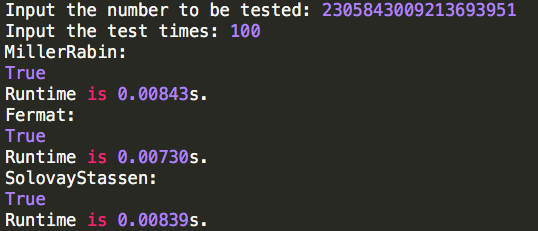
\includegraphics[height=4.62cm,width=10.76cm]{prime.png}
\caption{素性检验}
\label{img_prime}
\end{figure}

\subsection{算法实现}
\begin{breakablealgorithm}  
    \caption{Miller-Rabin算法}  
    \begin{algorithmic}[1] %每行显示行号  
        \Require 待测试数$n$,测试次数$times$  
        \Ensure $n$为合数,或者很可能为素数 
        \Function {MillerRabin}{$n, times$} 
            \State $power \gets 0$
            \State $rest \gets n - 1$
            \While {$rest \% 2 == 0$}
                \State $rest \gets rest >> 1$
                \State $power \gets power + 1$
            \EndWhile
            \For {each $i \in [1, times]$}
                \State $rand \gets RandomInt \in [2, n - 2]$
                \If {$rand^{rest}\quad$(mod $n$) $\in {1, n - 1}$}
                    \State continue
                \EndIf
                \State $actPower \gets rest$
                \For {each $j \in [0, power - 2]$}
                    \State $actPower \gets actPower * 2$
                    \If {$rand^{actPower}\quad$(mod $n$) $== n - 1$}
                        \State break
                    \EndIf
                \EndFor
                \If {$loop\;does\;not\;break$}
                    \State \Return $False$
                \EndIf
            \EndFor
            \State \Return $True$
        \EndFunction  
    \end{algorithmic}  
\end{breakablealgorithm} 
\begin{breakablealgorithm}  
    \caption{Fermat算法}  
    \begin{algorithmic}[1] %每行显示行号  
        \Require 待测试数$n$,测试次数$times$   
        \Ensure $n$为合数,或者很可能为素数
        \Function {Fermat}{$n, times$}  
            \For {each $i\in [1, times]$}
                \State $base \gets RandomInt \in [1, n - 1]$
                \State $gcd \gets gcd(n, base)$
                \If {gcd > 1}
                    \State \Return False
                \EndIf
                \If {$base^{n - 1}\quad$(mod $n$) $\neq 1$}
                    \State \Return $False$
                \EndIf
            \EndFor
            \State \Return $True$
        \EndFunction  
    \end{algorithmic}  
\end{breakablealgorithm} 

\begin{breakablealgorithm}  
    \caption{Solovay-Stassen算法}  
    \begin{algorithmic}[1] %每行显示行号  
        \Require 待测试数$n$,测试次数$times$   
        \Ensure $n$为合数,或者很可能为素数
        \Function {Jacobi}{$a, b$}
            \State $result = 1$
            \State $a = a \% b$
            \If {b == 1}
                \State \Return $result$
            \EndIf
            \While {$a \neq 0$}
                \While {$a \% 2 == 0$}
                    \State $a \gets a / 2$
                    \If {$b \% 8 \in {3, 5}$}
                        \State $result \gets -result$
                    \EndIf
                \EndWhile
                \State $a, b \gets b, a$
                \If {$a \% 4 == b \% 4 == 3$}
                    \State $result \gets -result$
                \EndIf
                \State $a \gets a \% b$
            \EndWhile
            \State \Return $result$
        \EndFunction
        \Function {SolovayStassen}{$n, times$}  
            \For {each $i\in [1, times]$}
                \State $base \gets RandomInt \in [2, n - 2]$
                \State $test1 \gets base^{\frac{n - 1}{2}}\quad$(mod $n$)
                \If {$test1 not \equiv \pm1$}
                    \State \Return $False$
                \EndIf
                \State $test2 \gets \Call{Jacobi}{base, n}$
                \If {$test1 \neq test2$}
                    \State \Return $False$
                \EndIf
            \EndFor
            \State \Return $True$
        \EndFunction  
    \end{algorithmic}  
\end{breakablealgorithm} 
\subsection{算法比较}
RM算法时间复杂度为$O(t\log \log n)$,Fermat算法时间复杂度为$O(t \log n)$,SS算法时间复杂度为$O(t \log n + t \log n) = O(t \log n)$。在$t$很大时,三个算法的错误几率都极小。








\section{$GF$域上的四则运算}
\subsection{$GF(2^8)$}
给定$GF(2)$上的$8$次不可约多项式$x^8 + x^4 + x^3 + x + 1$,可求得其生成元为$x + 1$。于是在$GF(2^8)$上,加法(减法)利用按位异或,乘法、除法、取逆都是使用打表的方式更加快捷,且不会消耗很多空间(3个长度为256的整数表)。本算法同时给出了移位异或的乘法方案,可以看出代码的繁琐。
\begin{breakablealgorithm}  
    \caption{$GF(2^8)$四则运算}  
    \begin{algorithmic}[1] %每行显示行号  
        \Require 二进制代表的两个多项式$num1, num2$  
        \Ensure $num1, num2$四则运算结果
        \Function {add}{$num1, num2$}  
            \State $num1, num2 \to int$
            \State \Return $num1 \oplus num2 \to str$
        \EndFunction  
        \Function {multiply}{$num1, num2$}
            \State $num2 \gets num2$反转
            \State $result \gets 0$
            \State $temp \gets int(num1)$
            \For {each $i \in [1, 8]$}
                \If {$num2[i] == 1$}
                    \State $result \gets result \oplus temp$
                \EndIf
                \If {temp [0] == 1}
                    \State $temp \gets (temp << 1)[1: ] \oplus 0x1B$
                \Else
                    \State $temp \gets (temp << 1)[1: ]$
                \EndIf
            \EndFor
            \State \Return $result \to str$
        \EndFunction
        
        \State $multi \gets [1]$
        \For {each $i \in [1, 254]$}
            \State $multi[i] \gets multi[i-1] << 1 \oplus multi[i-1]$
            \If {$multi[i] \& 0x100$}
                \State $multi[i] \gets multi[i] \oplus 0x11B$
            \EndIf
        \EndFor
        \State $arcMulti \gets multi$的反表
        \State $reverse \gets [0]$
        \For {each $i \in [1, 255]$}
            \State $reverse[i] \gets multi[(255 - arcMulti[i]) \% 255]$
        \EndFor
        \Function{tableMultiply}{$num1, num2$}
            \State \Return multi[(arcMulti[num1] + arcMulti[num2])\% 255]
        \EndFunction
        \Function{tableRev}{$num$}
            \State \Return $reverse[num]$
        \EndFunction
        \Function{divide}{$num1, num2$}
            \State $temp \gets$ \Call{tableRev}{$num2$}
            \State \Return \Call{tableMultiply}{$elm1, temp$}
        \EndFunction
    \end{algorithmic}  
\end{breakablealgorithm}
\subsection{$GF(2^8)$演示}
\subsection{测试样例}
\begin{figure}[htbp]
\centering
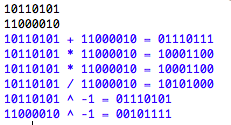
\includegraphics[height=5cm,width=9.24cm]{gf256.png}
\caption{$GF(2^8)$}
\label{img_gf256}
\end{figure}

\subsection{$GF(2^4)$}
与$GF(2^4)$情况相仿,选取4次不可约多项式为$x^4 + x^3 + 1$,其生成元为$x^2$。同样使用打表的方式获得乘法、除法、逆的结果,也给出了移位乘法的算法。
\begin{breakablealgorithm}  
    \caption{$GF(2^4)$四则运算}  
    \begin{algorithmic}[1] %每行显示行号  
        \Require 二进制代表的两个多项式$num1, num2$  
        \Ensure $num1, num2$四则运算结果
        \Function {add}{$num1, num2$}  
            \State $num1, num2 \to int$
            \State \Return $num1 \oplus num2 \to str$
        \EndFunction  
        \Function {multiply}{$num1, num2$}
            \State $num2 \gets num2$反转
            \State $result \gets 0$
            \State $temp \gets int(num1)$
            \For {each $i \in [1, 4]$}
                \If {$num2[i] == 1$}
                    \State $result \gets result \oplus temp$
                \EndIf
                \If {temp [0] == 1}
                    \State $temp \gets (temp << 1)[1: ] \oplus 0x9$
                \Else
                    \State $temp \gets (temp << 1)[1: ]$
                \EndIf
            \EndFor
            \State \Return $result \to str$
        \EndFunction
        
        \State $multi \gets [1]$
        \For {each $i \in [1, 14]$}
            \State $multi[i] \gets multi[i-1] << 1 $
            \If {$multi[i] \& 0x10$}
                \State $multi[i] \gets multi[i] \oplus 0x19$
            \EndIf
            \State $multi[i] \gets multi[i] << 1 $
            \If {$multi[i] \& 0x10$}
                \State $multi[i] \gets multi[i] \oplus 0x19$
            \EndIf
        \EndFor
        \State $arcMulti \gets multi$的反表
        \State $reverse \gets [0]$
        \For {each $i \in [1, 15]$}
            \State $reverse[i] \gets multi[(15 - arcMulti[i]) \% 15]$
        \EndFor
        \Function{tableMultiply}{$num1, num2$}
            \State \Return multi[(arcMulti[num1] + arcMulti[num2])\% 15]
        \EndFunction
        \Function{tableRev}{$num$}
            \State \Return $reverse[num]$
        \EndFunction
        \Function{divide}{$num1, num2$}
            \State $temp \gets$ \Call{tableRev}{$num2$}
            \State \Return \Call{tableMultiply}{$elm1, temp$}
        \EndFunction
    \end{algorithmic}  
\end{breakablealgorithm}
\subsection{$GF(2^4)$演示}
\subsection{测试样例}
\begin{figure}[htbp]
\centering
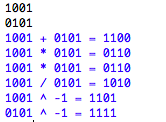
\includegraphics[height=6.1cm,width=8.3cm]{gf16.png}
\caption{$GF(2^4)$}
\label{img_gf16}
\end{figure}







\section{原根生成算法}% finish
\subsection{算法简介}
 先求得Euler函数$\phi(n)$,再对$n$进行素因子分解。对每个即将测试的$g$,只要所有的$g^{\frac{\phi(n)}{p}}\neq 1 \quad$ (mod $n$),且$g^{\phi(n)} \equiv 1 \quad$ (mod $n$)就说明$g$是原根。
\subsection{测试样例}
\begin{figure}[htbp]
\centering
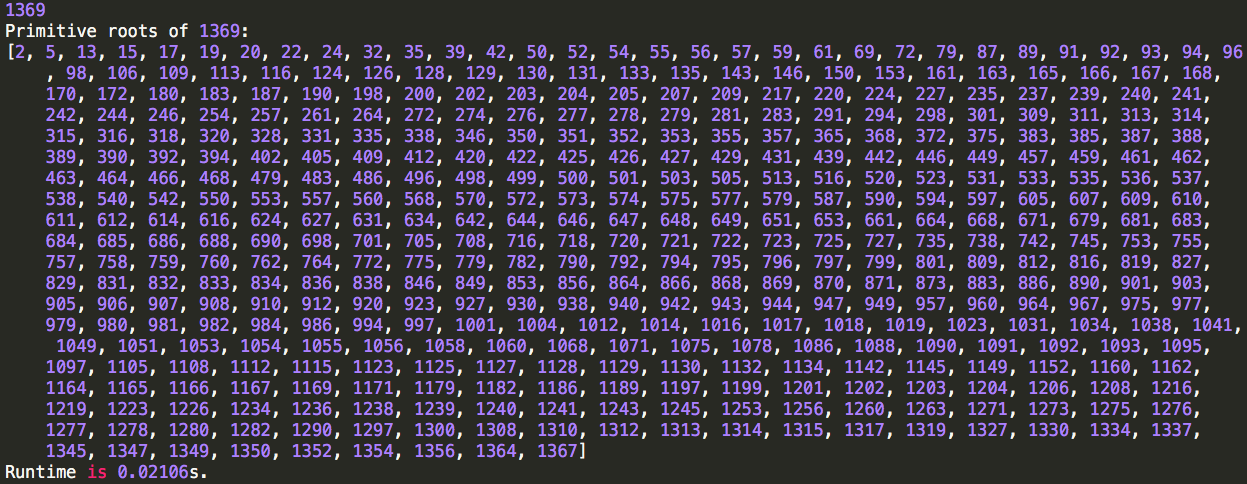
\includegraphics[height=4.84cm,width=12.47cm]{root.png}
\caption{原根}
\label{img_roots}
\end{figure}
\subsection{算法实现}
\begin{breakablealgorithm}  
    \caption{计算Euler函数}  
    \begin{algorithmic}[1] %每行显示行号  
        \Require $n$  
        \Ensure $n$的Euler函数值
        \Function {phi}{$n$}
            \State $result \gets n$
            \State $i \gets 2$
            \While {$i^2 \leqslant n$}
                \If {$n \% i == 0$}
                    \While {$n \% i == 0$}
                        \State $n \gets n / i$
                    \EndWhile
                    \State $result \gets result - result / i$
                \EndIf
                \State $i \gets i + 1$
            \EndWhile
            \If {n > 1}
                \State $result \gets result - result / n$
            \EndIf
            \State \Return $result$
        \EndFunction
    \end{algorithmic}  
\end{breakablealgorithm} 
\begin{breakablealgorithm}  
    \caption{原根生成算法}  
    \begin{algorithmic}[1] %每行显示行号  
        \Require $n$  
        \Ensure $n$的原根
        \Function {primitive}{$n$}  
            \State $roots, factors \gets []$
            \If {$n == 2$}
                \State \Return $1$
            \EndIf
            \State $euler \gets $\Call{phi}{$n$}
            \State $temp \gets euler$
            \For {each $i \in [2, \sqrt{n}]$}
                \If {$n \% i == 0$}
                    \State $factors.append(i)$
                    \While {$temp \% i == 0$}
                        \State $temp \gets temp / i$
                    \EndWhile
                \EndIf
            \EndFor
            \If {n > 1}
                \State $factors.append(n)$
            \EndIf
            \For {each $g \in [2, n]$}
                \For {each $p \in factors$}
                    \If {$g^{\frac{euler}{p}}\quad$(mod $n$)$ == 1 \; or \; g^{euler}\quad$(mod $n$)$ \neq 1$}
                        \State break
                    \EndIf
                    \If {$loop\;does\;not\;break$}
                        \State $roots.append(g)$
                    \EndIf
                \EndFor
            \EndFor
            \State \Return $roots$
        \EndFunction  
    \end{algorithmic}  
\end{breakablealgorithm} 








\section{本原多项式的生成}
\subsection{简介}
唯一分解环上系数均互素的多项式为本原多项式。
\textbf{由于本实验根本没有说明具体在哪个唯一分解环上如何生成次数为几的本原多项式,因此本算法采用整数环为唯一分解环,采用随机数方式生成。}
\subsection{算法}
\begin{breakablealgorithm}  
    \caption{本原多项式生成}  
    \begin{algorithmic}[1] %每行显示行号  
        \Require 次数$n$  
        \Ensure 一个随机生成的$n$次本原多项式
        \Function {generate}{$n$}
            \State $factors \gets []$
            \State $factors.append(randint(1, 50))$
            \State $gcd \gets factors[0]$
            \For {each $i \in [1, n]$}
                \While {$True$}
                    \State $temp \gets randint(1, 50)$
                    \State $tgcd \gets $\Call{gcd}{$temp, gcd$}
                    \If {$tgcd == 1$}
                        \State $gcd \gets tgcd$
                        \State $factors.append(temp)$
                        \State break
                    \EndIf
                \EndWhile
            \EndFor
            \State \Return $factors$
        \EndFunction
    \end{algorithmic}  
\end{breakablealgorithm} 
\subsection{测试样例}
\begin{figure}[htbp]
\centering
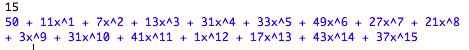
\includegraphics[height=1.50cm,width=14.07cm]{generate.png}
\caption{本原多项式}
\label{img_gemerate}
\end{figure}




\section{感想}
我希望实验要求能明确一点。\textbf{如果出题者不站在解题者的角度思考问题,则这个要求不可能是完备而清晰的。}对于本原多项式和有限域的四则运算的讲解太不清晰了,导致很多内容需要我花很多时间来弄明白。事实上,关于本原多项式实验的确切要求我直到此刻还没有弄懂。

希望老师能提前给出实验内容,以便于预习。此外,本次实验报告提交时间有些早了。

尽管如此,我还是学会了很多内容,无论是数学、编程还是排版。希望这门课能变得更好。
\end{document}